\documentclass[11pt,xcolor=svgnames]{beamer}
\usepackage{dsfont,natbib,setspace,changepage,multirow}
\mode<presentation>

% replaces beamer foot with simple page number
\setbeamertemplate{navigation symbols}{}
%\setbeamerfont{frametitle}{series=\bfseries}
\setbeamercolor{frametitle}{fg=Black}

\setbeamertemplate{footline}{
   \raisebox{5pt}{\makebox[\paperwidth]{\hfill\makebox[20pt]{\color{gray}\scriptsize\insertframenumber}}}}

\graphicspath{{/Users/mtaddy/Dropbox/inputs/}}
\usepackage{algorithm}
\usepackage{algorithmic}

% colors
\newcommand{\theme}{\color{Maroon}}
\newcommand{\bk}{\color{black}}
\newcommand{\rd}{\color{DarkRed}}
\newcommand{\fg}{\color{ForestGreen}}
\newcommand{\bl}{\color{blue}}
\newcommand{\gr}{\color{black!50}}
\newcommand{\sg}{\color{DarkSlateGray}}
\newcommand{\nv}{\color{Navy}}
\setbeamercolor{itemize item}{fg=gray}

% common math markups
\newcommand{\bs}[1]{\boldsymbol{#1}}
\newcommand{\mc}[1]{\mathcal{#1}}
\newcommand{\mr}[1]{\mathrm{#1}}
\newcommand{\bm}[1]{\mathbf{#1}}
\newcommand{\ds}[1]{\mathds{#1}}
\newcommand{\indep}{\perp\!\!\!\perp}
\def\plus{\texttt{+}}
\def\minus{\texttt{-}}

% spacing and style shorthand
\setstretch{1.1}

\begin{document}

\setcounter{page}{0}
{% \usebackgroundtemplate{\includegraphics[height=\paperheight]{phoenix}}
\begin{frame}[plain]
\begin{center}

{\bf \LARGE \theme }

\vskip .25cm
{\bf \LARGE \theme Empirical Bayesian Forests }

\vskip 1cm
Matt Taddy,  Chicago Booth

\vskip .1cm
with Chun-Sheng Chen, Jun Yun, and Mitch Wyle at eBay


\vfill
{\texttt{faculty.chicagobooth.edu/matt.taddy/research}}

\end{center}
\end{frame} }


\begin{frame}
{What is a Decision Tree?}

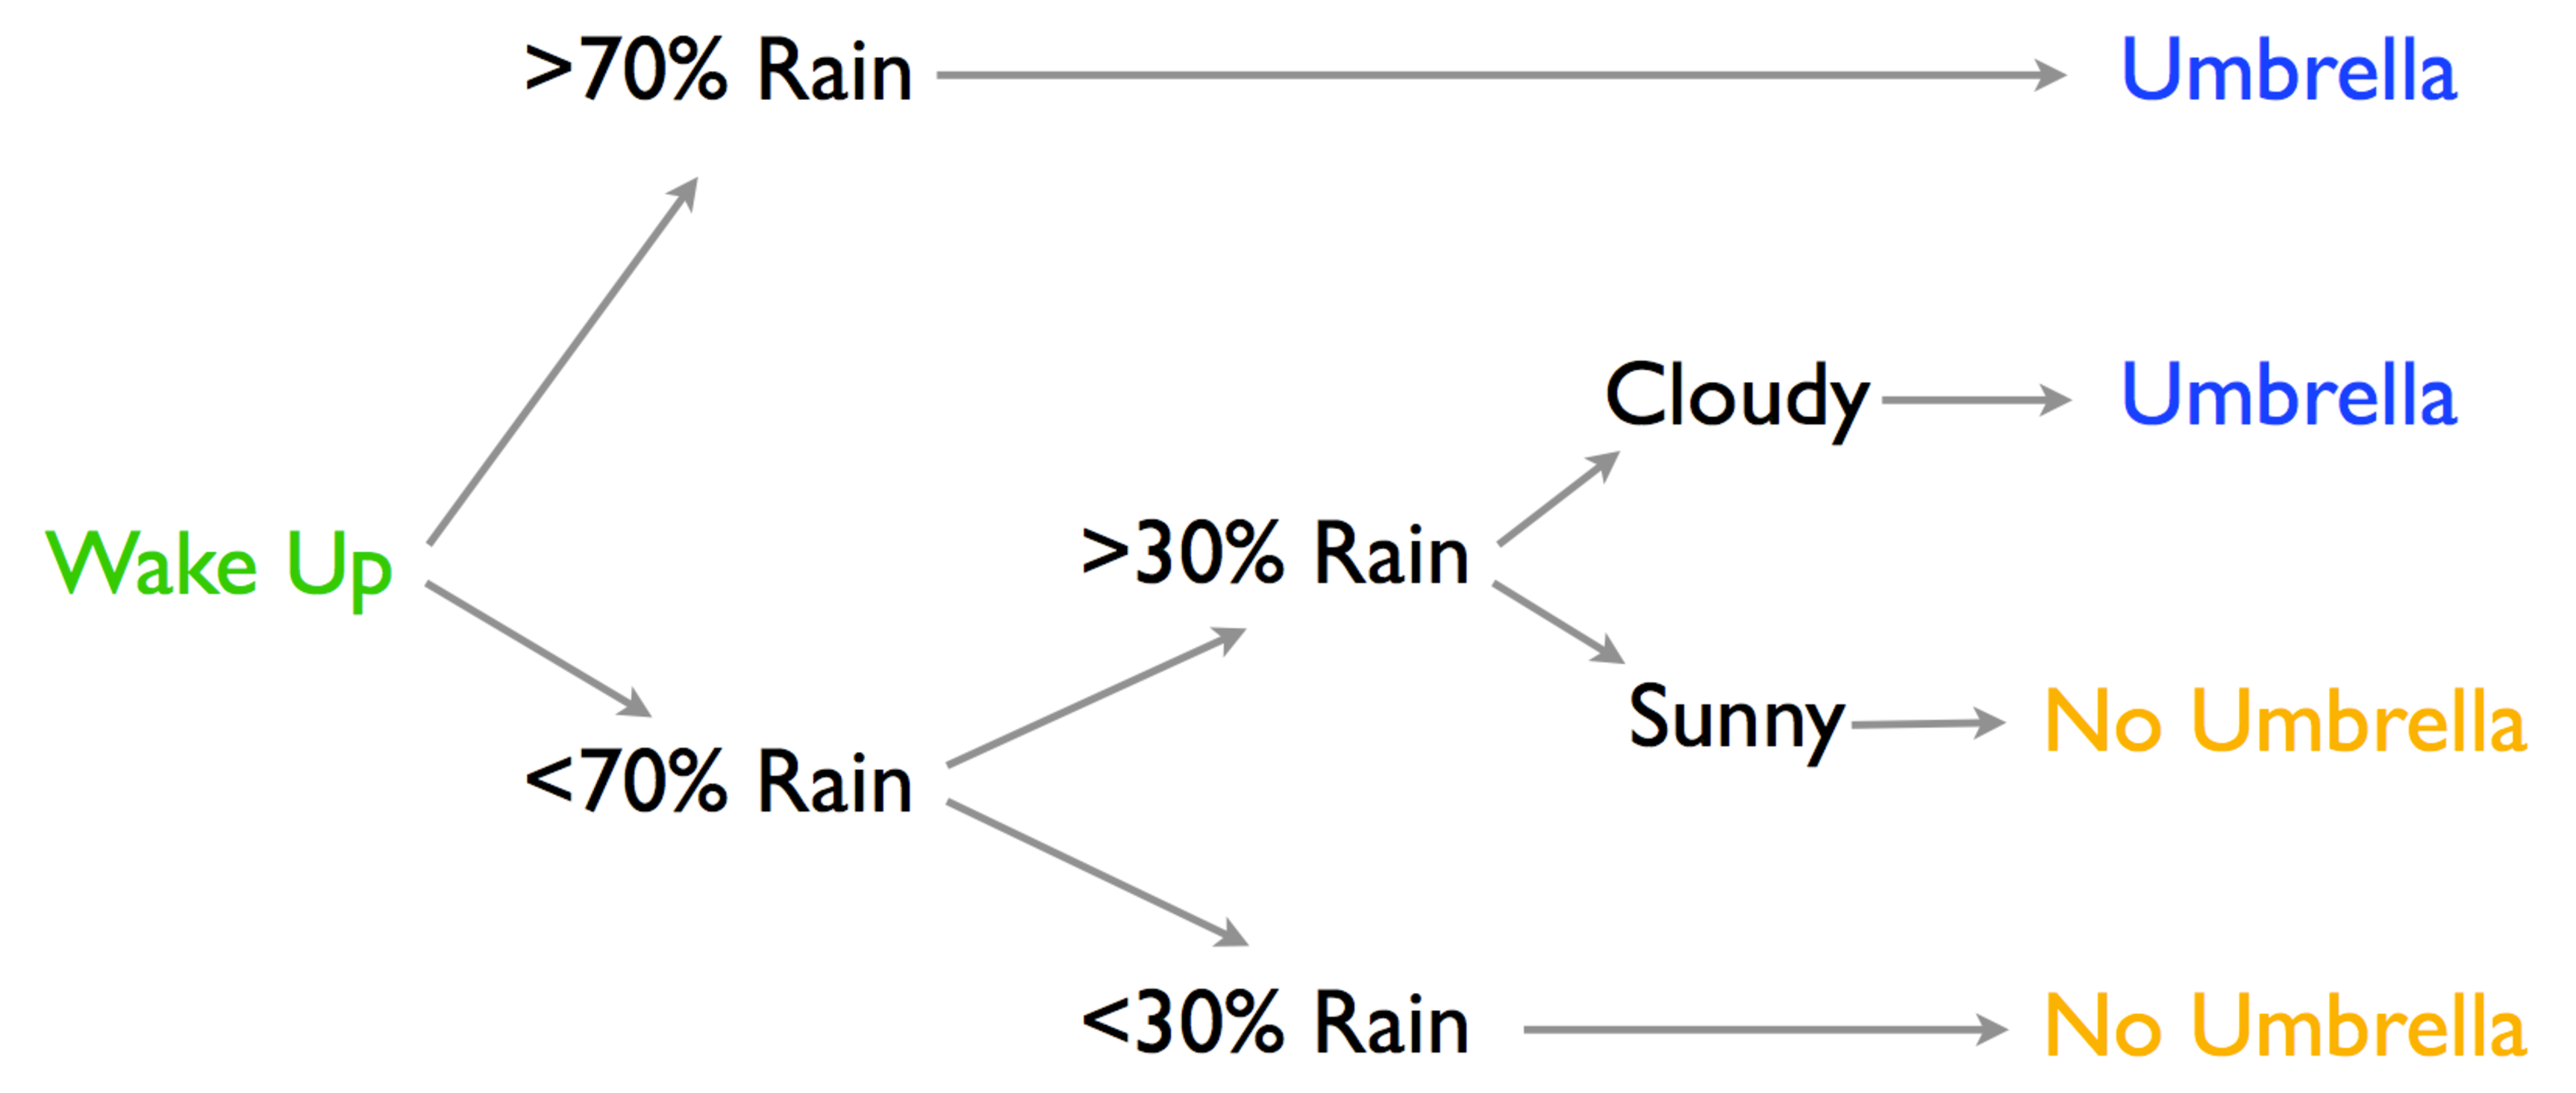
\includegraphics[width=4.25in]{../../bigdata/graphs/umbrella}


\vskip .3cm
\bk Tree-logic uses a series of steps to come to a conclusion.\\
 The trick is to have mini-decisions combine for good choices.
\\ Each decision is a node, and the final prediction is a {\theme
  leaf node}

\end{frame}


\begin{frame}

{\bf \theme Neighborhoods: \bk Parents, Siblings, Children, and Leaves}

\vskip -.25cm
\begin{columns}

\column{1.75in}

\vskip -.1cm
\begin{equation*}~~~~
\begin{array}{ccccc}
& &  \hskip -1cm P(\eta) &&\\
& & \hskip -1cm \swarrow ~~~\searrow &&\\
&  \hskip -.5cm\eta & & \hskip -.5cm S(\eta)&\\
& \hskip -.5cm \swarrow~~~\searrow & & &\\
C_{l}(\eta) & & \hskip -.3cm  C_r(\eta) & &
\end{array}
\end{equation*}

\column{2.75in}

\vskip .5cm

Every node has a {\it parent} (except root).

\vskip .5cm
Nodes sharing  parents are {\it siblings}.

\vskip .5cm
Each node can have its own {\it children}.
\end{columns}


\vskip .5cm
{After descending through splits, {\nv leaf nodes} hold a
  data subset}

\vskip -.25cm
\begin{equation*}
\begin{array}{ccccc}
& &  \hskip -2.2cm x_i = 0 &&\\
& & \hskip -2.3cm \swarrow ~~~\searrow &&\\
&  \hskip -.8cm x_j = 2 & & \hskip -2.3cm \{\bm{x}: x_i>0\}&\\
& \hskip -.7cm \swarrow~~~\searrow & & &\\
\{\bm{x}: x_i \leq  0, x_j \leq  2\}& & \hskip -.5cm \{ \bm{x}: x_i \leq 0, x_j>2 \}& &
\end{array}
\end{equation*}

\vskip -.5cm
\end{frame}

\begin{frame}


{\bf  Estimation of Decision Trees}

\vskip .5cm  We maximize data likelihood 
   by thinking recursively: 

~~~~~ \bk Split the data into two different decisions about $y$. 

\hfill Take each new partition and split again.

\vskip .5cm
\bk
{\bf \theme Growing \bk your tree  with the \theme CART \bk
  algorithm:}

\begin{itemize}\bk
\item Find the split location in $\bm{x}$ that minimizes deviance.
\begin{itemize}
\item[\gr $\bullet$] $\hat{y}_i$ or $\hat{p}_i$ change depending on whether $x_i <
  x_{\text{split}}$.
\end{itemize}
\item You then grow the tree at this point
\begin{itemize}
\item[\gr $\bullet$]  Each new child node contains a subset of the data.
\end{itemize}
\item View each child as a new dataset, and try to grow again.
\begin{itemize}
\item[\gr $\bullet$] Stop splitting/growing when there are some fixed minimum 
number of observations in each leaf node. 
\end{itemize}
\end{itemize}

\vskip -.25cm
\end{frame}


\begin{frame}

{\bf \theme Random Forests}

\vskip .5cm \bk
CART is an effective way to choose a single tree, but often there are
many possible trees that fit the data similarly well.


\vskip .5cm \nv
An alternative approach is to make use of {\nv random forests}.

\bk
\vskip .25cm
$\bullet$ Sample $B$ subsets of the data {\tt +} variables: \\ ~~~e.g., 
observations $1,5,20,...$ and inputs $2,10,17,...$

\vskip .2cm
$\bullet$ Fit a tree to each subset, to get $B$ fitted trees is $\mc{T}_b$.

\vskip .2cm
$\bullet$
Average prediction across trees:

\vskip .1cm
 ~~~~ -  for regression average $\ds{E}[y|\bm{x}] = \frac{1}{B}\sum_{b=1}^B \mc{T}_b(\bm{x})$.

 \vskip .1cm
 ~~~~ -  for classification let $\{\mc{T}_b(\bm{x})\}_{b=1}^B$ vote on $\hat y$.

\vskip .25cm
{\gr The observation resample is usually {\it with-replacement}, so that this is taking the {\it average of bootstrapped trees} (i.e., `bagging')}

\end{frame}

\begin{frame}

{\theme \bf nonparametric statistics }

\vskip .25cm
1: Find some statistic that matters for your problem, \\~~~~regardless of the `data generating process' (DGP).

\vskip .25cm
2: Derive the distribution for this stat under minimal assumptions.

\vskip .5cm
For (2): say $\bm{z}_l = \{\bm{x}_l,y_l\}$ is a possible data point. Then
\[
\mr{p}(\bm{Z}) = \sum_{l=1}^L \omega_l \ds{1}{[\bm{Z} = \bm{z}_l]}
\]
where $L$ is a {\it large} number of possible values.
\begin{itemize}
\item Use sample as stand-in for the $L$  points.
\item Bayesian  model for the $\omega_l$ weights.
\item {\it This is essentially a bootstrap.}
\end{itemize}

\end{frame}

\begin{frame}[fragile]


Our statistic of interest is the CART fit...

\vskip .5cm
\begin{center}
{\sc Bayesian Forest}
\begin{algorithmic}
   \FOR{$b=1$ {\bfseries to} $B$}
   \STATE draw $\boldsymbol{\theta}^b \stackrel{iid}{\sim} \mathrm{Exp}(\mathbf{1})$
   \STATE run weighted-sample CART to get $\mathcal{T}_b = \mathcal{T}(\boldsymbol{\theta}^b)$
   \ENDFOR
\end{algorithmic}
\end{center}

\vskip .5cm
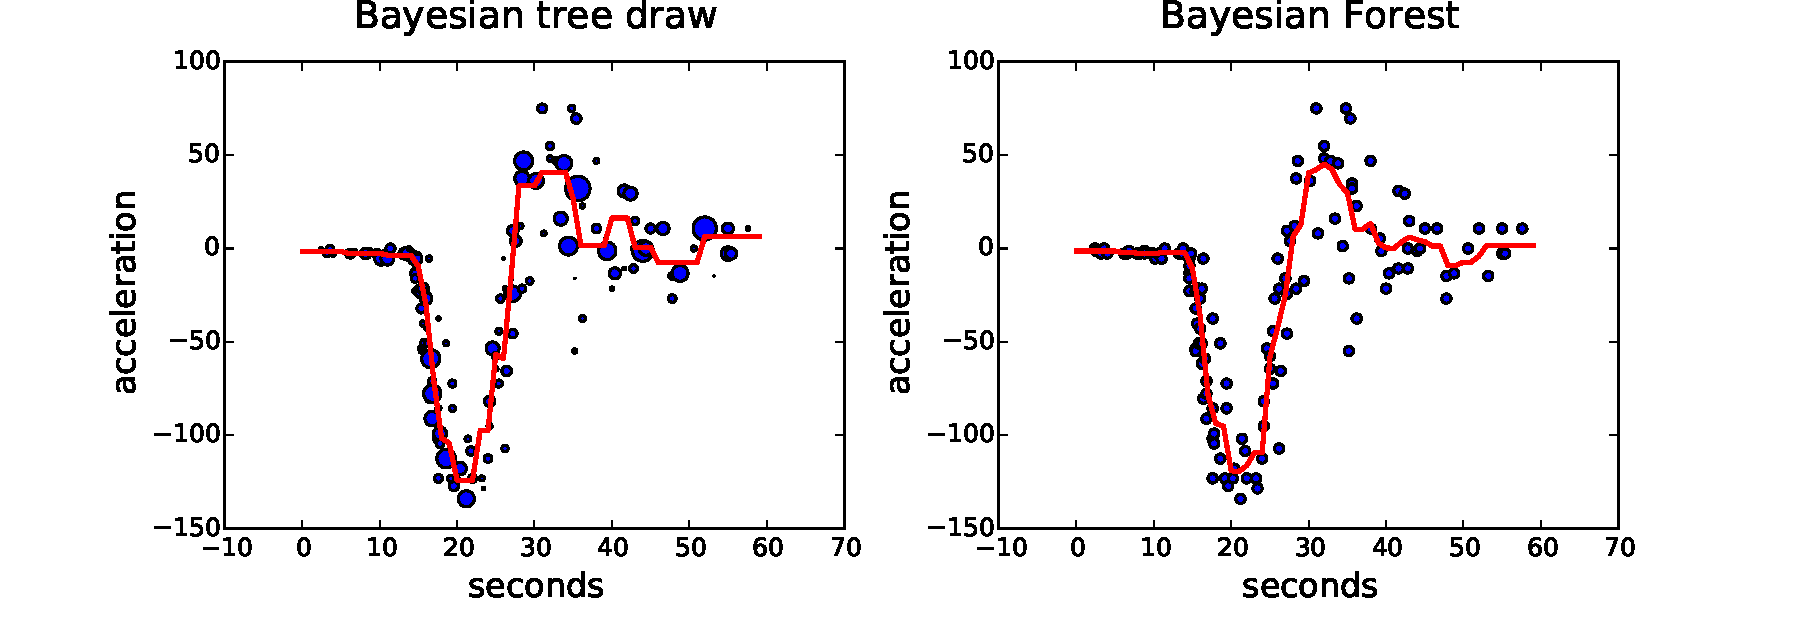
\includegraphics[width=.95\textwidth]{../graphs/mcycle}   

\end{frame}

\begin{frame}


Given this expression of forests as a posterior, \\we can start talking about {\it variance}

\vskip .5cm
For the data at a given node on the
sample CART tree, the probability that the next split for a posterior
DGP realization  matches the sample split location is
\begin{equation*}
\mathrm{p}\left(\text{split matches sample CART}\right) \gtrsim 1 - \frac{p}{\sqrt{n}} e^{-n},
\end{equation*}
where $p$ is the number of possible split locations and $n$ the number of observations on the current node.  

\vskip .5cm So things are pretty stable (until they aren't).
\end{frame}

\begin{frame}

{\bf California Housing Data}

\vskip .5cm

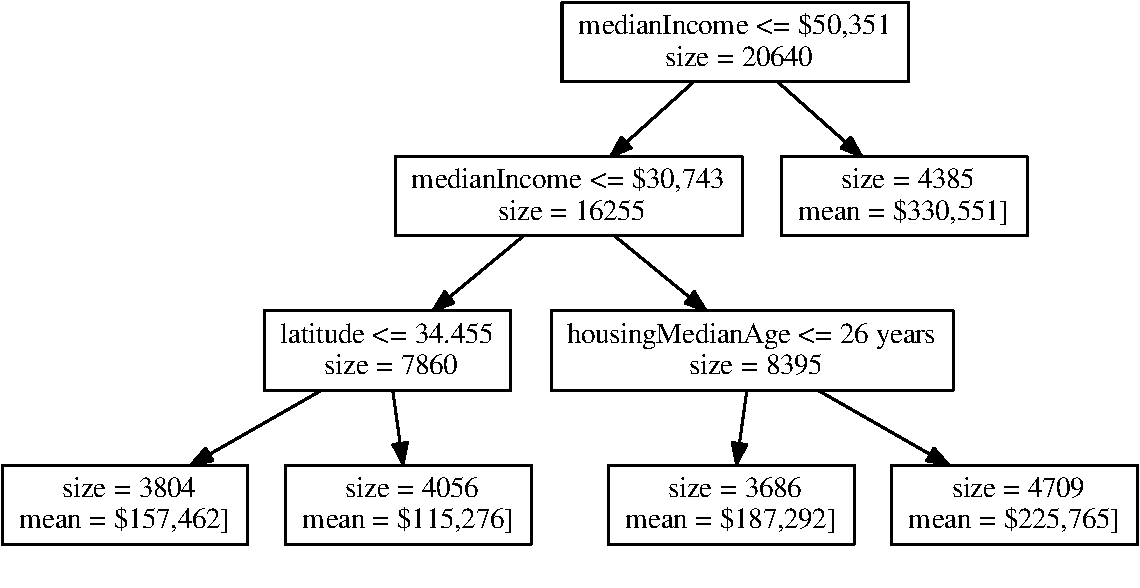
\includegraphics[width=\textwidth]{../graphs/ca_trunk}

\vskip .5cm

\hfill 20k observations.

\end{frame}

\begin{frame}

\begin{columns}

\begin{column}{2.15in}
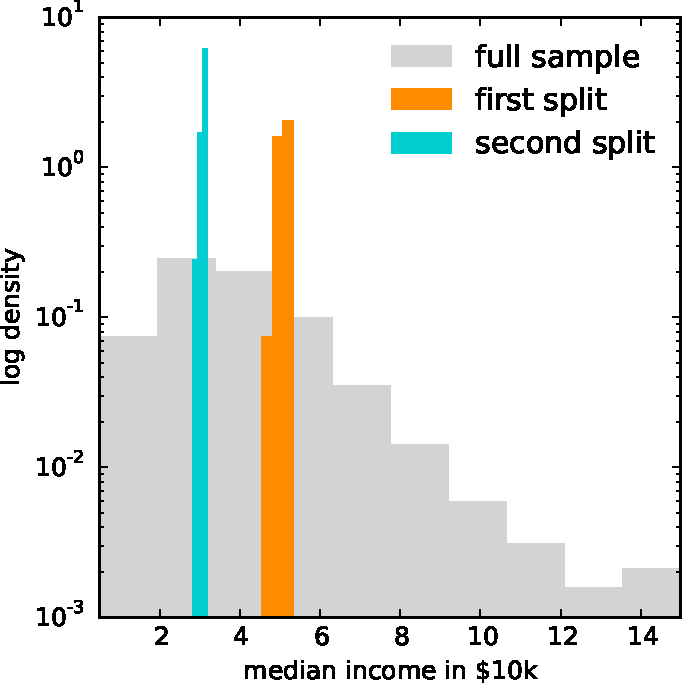
\includegraphics[width=2.5in]{../graphs/ca_splits}
\end{column}

\begin{column}{2in}
\begin{itemize}
\item sample tree occurs 62\% \\of the time.  
\vskip .5cm
\item 90\% of  trees split on income twice, \\and then latitude. 

\vskip .5cm
\item 100\% of trees have 1st 2 splits on median income.  
\end{itemize}
\end{column}

\end{columns}


\vskip 1cm
~~~~~~~~~~~~~~~~~~So trees are stable, at the trunk.
\vskip -1cm

\end{frame}

\begin{frame}

{\bf A big data problem}

\vskip .5cm
RFs are expensive when data is too big to fit in memory.

\vskip .5cm
Subsampling forests (fitting CART on {\it without replacement} samples)
leads to a big drop in performance.

\vskip .5cm
{\theme But wait:}  if the trunks are stable, can we just fit that once and then fit forests at each branch?

\vskip .5cm
This is classic Empirical Bayes: fix higher levels in a {\it hierarchical model}, and direct your machinery at learning the hard bits.

\end{frame}

\begin{frame}

{\bf Emperical Bayesian Forests}

\vskip .5cm
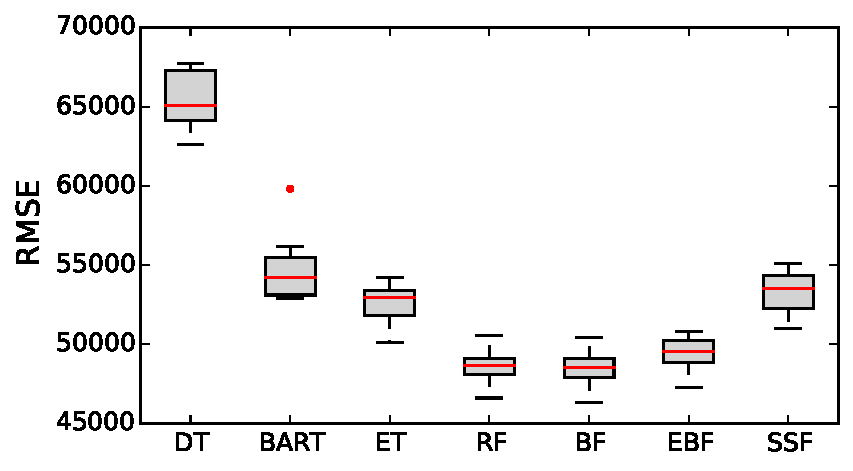
\includegraphics[width=.95\textwidth]{../graphs/ca_rmse}

\vskip .5cm
Since the trunks in a full forest are all similar, EBF and BF give nearly the same results.  {\it SSF does not.}


\end{frame}


\begin{frame}

EBFs work all over the place

\begin{columns}
\begin{column}{2in}
\begin{center}
{\bf ~~~~~beer}
\end{center}

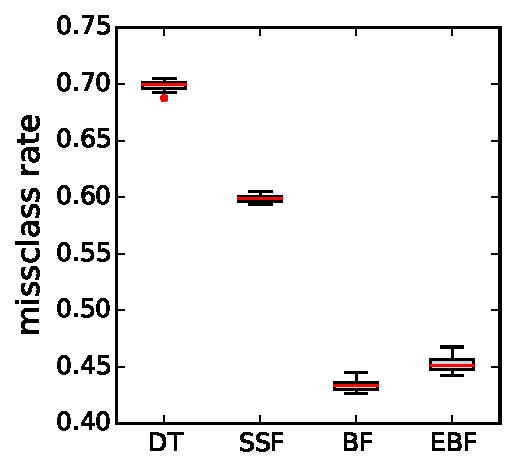
\includegraphics[width=2in]{../graphs/beer}
\end{column}

\begin{column}{2in}
\begin{center}
{\bf ~~~~~~~wine}
\end{center}

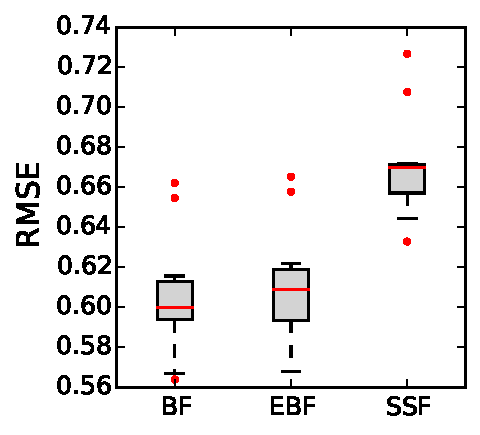
\includegraphics[width=2in]{../graphs/wine}
\end{column}
\end{columns}

\vskip .5cm
\hfill Predicting beer choice from demographics, \\\hfill and wine rating from chemical profile
\end{frame}

\begin{frame}


{\bf \theme EBFs at eBay: \bk predicting Bad Buyer Experiences}

\vskip .25cm

\begin{itemize}
\item trunk can be fit in distribution using Spark \texttt{MLLib}.
\item this trunk  acts as a sorting function to map observations \\to 
separate locations corresponding to each branch.
\item Forests are then fit on a machine for each branch.  
\end{itemize}

\vskip .5cm

On 12 million transactions,  EBF with 32 branches yields a 1.3\% drop in misclassification over the SSF alternatives.  

\vskip .5cm
This amounts to more than 20,000 extra detected \\BBE occurrences over this short time window.

\end{frame}

\begin{frame}

{\theme\bf  The key to big data} 

\vskip .5cm Use plug-in estimates for the stuff that is easy to measure.

\vskip .15cm Partition conditional on these plug-ins.

\vskip .15cm   Direct the full data towards the stuff that is tough to learn.

\vskip 1.5cm
\begin{center}
\Huge
Thanks!
\end{center}

\end{frame}

\end{document}






























